\section{Problem and motivation}
\label{sec:motivation}
A coding agent receives an issue and a repository and produces a patch.
Its trajectory records actions, observations, and the outcome. ContextGraph
builds an experience graph $G$ from completed trajectories, retrieves guidance
for each new task, and updates $G$ afterward. The goal is to accumulate useful
repair experience across tasks and repositories.

\paragraph{A debugging decision that transfers.}
In Django Trac \#33018, empty query results are mishandled under negation.
A failed \texttt{python-statemachine} attempt had spent its effort setting
up a full Django application; its lesson was to isolate the failure before
investing in framework setup. A successful \texttt{sievelib} trajectory also
supported reproducing the failure before editing. Guided by these experiences,
the agent traced the exception to \texttt{Exists.as\_sql()}, corrected its
handling, and added a regression test. The no-memory attempt made broad
formatting changes without fixing the bug. The transferable content was the
investigation strategy and warning; the agent derived the local implementation.

\paragraph{From advice to a concrete check.}
Remembered guidance also needs to be applied to the current operation.
Figure~\ref{fig:concept} illustrates another Django case: a historical requirement
becomes a check by combining its input condition with the current query.
Section~\ref{sec:behavior-analysis} compares separate and composed checks.

\begin{figure}[!htbp]
\centering
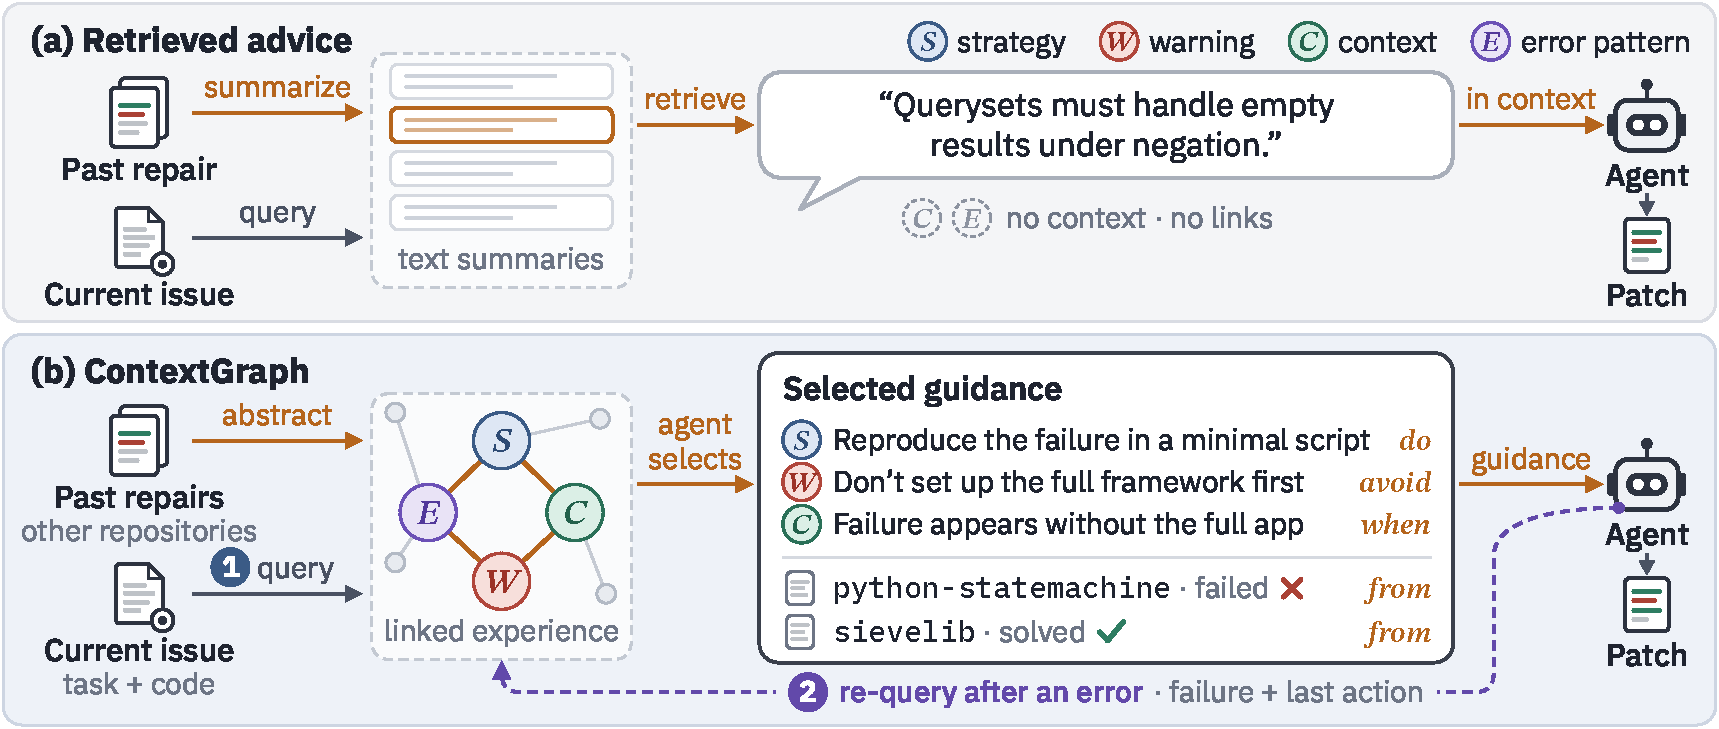
\includegraphics[width=\linewidth]{figures/contextgraph-design/fig1-concept.pdf}
\caption{Django12663 behavioral study comparing (a) a requirement supplied as text
with (b) linked context used to combine a historical range type with the
current query and obtain execution feedback for the next edit.}
\label{fig:concept}
\end{figure}

\section{ContextGraph: memory for planning, recovery, and learning}
\label{sec:method}
ContextGraph connects experience abstraction, graph retrieval, and memory
access. The same process builds the initial graph and incorporates completed
tasks (Figure~\ref{fig:experience-memory}).

\begin{figure}[!htbp]
\centering
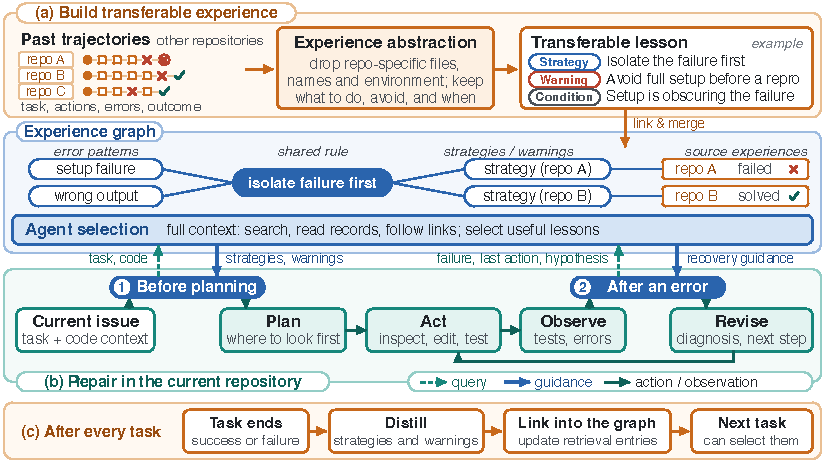
\includegraphics[width=\linewidth]{figures/experience-architecture/fig3-contextgraph.pdf}
\par\smallskip
\begin{tikzpicture}[>=Stealth, node distance=0.18cm,
  cgstep/.style={draw=blue!55!black, rounded corners=2pt, fill=blue!4,
    align=center, font=\scriptsize, minimum height=0.63cm, inner sep=4pt}]
\node[cgstep,text width=2.6cm] (task) {Complete a task\\success or failure};
\node[cgstep,text width=2.7cm,right=of task] (learn) {Distill experience\\strategies and warnings};
\node[cgstep,text width=2.45cm,right=of learn] (update) {Update the graph\\and retrieval entries};
\node[cgstep,text width=2.75cm,right=of update] (next) {Next task\\retrieves new experience};
\draw[->,thick,blue!65!black] (task) -- (learn);
\draw[->,thick,blue!65!black] (learn) -- (update);
\draw[->,thick,blue!65!black] (update) -- (next);
\end{tikzpicture}
\caption{ContextGraph's experience-memory architecture. Past trajectories
supply strategies and warnings linked to source context. The agent retrieves
guidance using its full context before planning and after errors. After every task, successful and
failed trajectories update the graph; the added experience is immediately
available to subsequent tasks. Graph links illustrate the organization.}
\label{fig:experience-memory}
\end{figure}

\subsection{Experience abstraction: retain the useful decision}
\label{sec:experience-abstraction}
A language model extracts lessons from the task, actions, errors, and outcome.
Each lesson records an action or warning, its applicability conditions, and
source context. Abstraction removes repository-specific names while retaining
the decision and its reason: the failed framework setup becomes advice to
isolate the bug first.

Strategies link to their source trajectories and shared rules; rules and
experiences link to the errors they address or encounter. These connections
preserve the common lesson and its supporting observations, including warnings
from failures and strategies from successful repairs.

\subsection{Agent-directed selection: find useful experience}
\label{sec:experience-retrieval}
The agent uses its full current context---the issue, inspected code, previous
actions, and observed failures---to decide which memories can help. It can
search the entire experience pool, open source records, follow links between
errors and strategies, and refine its search as its diagnosis changes.
Semantic and keyword search provide entry points; the agent selects the
useful lessons rather than receiving a fixed top-$k$ list.

The graph keeps each strategy connected to its applicability context and
supporting experience. The agent uses these connections to judge relevance,
then applies selected strategies and warnings through local reproductions,
edits, and tests. Appendix~\ref{sec:agentic-retrieval} details the selection
workflow.

\subsection{Memory access and updates: connect repair to learning}
\label{sec:experience-access}
\paragraph{Before planning.}
The agent searches memory using the issue and its full available code context.
Strategies guide where to investigate, how to reproduce the failure, and
which checks to prioritize; warnings identify costly approaches to avoid.

\paragraph{After an error.}
A failed command, reproduction, or test adds to the agent's current context:
the observed error, recent action, relevant files, and current hypothesis.
Retrieval now supports diagnosis and revision. The agent applies the guidance
through its repository tools and uses the next observation to decide how to proceed.

\paragraph{After each task.}
ContextGraph abstracts both successful and failed trajectories, links the
new lessons to existing experience, and updates their retrieval entries.
Outcomes here come from agent-visible observations, not official test feedback.
The added experience is immediately available to subsequent tasks, closing
the learning loop in Algorithm~\ref{alg:contextgraph}.

\begin{algorithm}[!htbp]
\caption{ContextGraph across a stream of coding tasks}
\label{alg:contextgraph}
\small
\begin{tabular}{@{}p{0.96\linewidth}@{}}
\textbf{Input:} initial trajectories $H$, coding tasks $q_1,\ldots,q_T$.\\
\textbf{Output:} candidate patches and an updated experience graph $G$.\\
1. Extract strategies and warnings from $H$; build $G$ and its retrieval entries.\\
2. \textbf{For each} task $q_t$ in issue creation-time order:\\
\quad a. Use the full task context to search $G$ and select guidance for planning.\\
\quad b. Execute investigation, editing, and testing actions; record the trajectory.\\
\quad c. After an error, search again with the updated full context; revise the plan.\\
\quad d. Continue the repair loop until the task ends or its budget is exhausted.\\
\quad e. Distill experience from the trajectory and agent-visible outcomes.\\
\quad f. Update $G$ and retrieval entries; expose the new experience to later tasks.\\
\end{tabular}
\end{algorithm}
